\documentclass[twocolumn]{article}
\usepackage{graphicx}
\usepackage{hyperref}
\usepackage{graphicx}
\usepackage{float} % Helps with precise image placement

\title{C Spreadsheet Project}
\author{Swara, Ayachi}
\date{}

\begin{document}

\maketitle

\section{Introduction}

Brief description of what the project does.

This project is a command-line spreadsheet written in C, similar to Microsoft Excel but with a command-line interface. A grid of cells is created by the program, where each cell stores an integer value. Users can interact with the spreadsheet by typing commands: they can write cell values directly or provide references to other cells and perform arithmetic operations.

The program is launched using:

\texttt{./sheet r c}

where \texttt{r} is the number of rows and \texttt{c} is the number of columns.

At any given instant, only a $10\times10$ portion of the sheet is visible to the user. Scroll commands allow the user to move to different parts of the sheet. The program keeps accepting commands and executing them until the user enters \texttt{q} to exit.

\section{Challenges and Design Decisions}

In developing this spreadsheet, we encountered several architectural challenges. Below we detail the engineering trade-offs and design decisions made to ensure the program remains performant and robust.

\subsection{Memory Optimization and Performance (Chunking)}
A major challenge was the potential for extremely high memory usage and slow execution times when handling the maximum allowed grid size (ZZZ999). 
\begin{itemize}
    \item \textbf{The Challenge:} Allocating a flat 2D array for millions of cells would lead to a massive memory footprint, most of which would likely be empty (sparse).
    \item \textbf{The Solution:} We implemented a \textbf{Chunked Memory Management} system. Instead of allocating all cells upfront, we use a two-level pointer system that allocates "chunks" of 1024 cells only when a cell within that range is accessed.
    \item \textbf{Why this works:} This approach is highly compatible with \textbf{L1/L2 Caching}. By keeping 1024 cells in a contiguous block, the CPU can load a chunk into cache memory once, making operations on neighboring cells significantly faster due to spatial locality.
\end{itemize}

\subsection{Dependency Tracking and Graph Structure}
Spreadsheets are essentially Directed Graphs. Tracking which cells depend on each other was a core difficulty because a single cell might have multiple parents (dependencies) and multiple children (dependents).
\begin{itemize}
    \item \textbf{Design Decision:} We included both a \texttt{dependencies} list and a \texttt{dependents} list in our \texttt{Cell} struct. 
    \item \textbf{The Benefit:} Keeping both lists allows for bidirectional traversal. We use the \texttt{dependencies} list during formula evaluation to know what values to fetch, and we use the \texttt{dependents} list to "push" updates forward when a cell's value changes.
\end{itemize}

\subsection{Circular Formula Detection}
One of the most dangerous edge cases in a spreadsheet is a circular reference (e.g., $A1=B1+1$ and $B1=A1+1$). 
\begin{itemize}
    \item \textbf{Our Approach:} We chose to perform cycle detection \textbf{at the moment of assignment}. 
    \item \textbf{Logic:} Before finalizing a new formula, we run a Depth First Search (DFS) using the \texttt{visited} and \texttt{in\_stack} flags. If we encounter a node already in the current recursion stack, we identify a back-edge (a cycle). This allows us to block the operation immediately and alert the user rather than letting the program enter an infinite loop.
\end{itemize}

\subsection{Push Model vs. Dirty Flagging}
We debated between using "Dirty Flagging" (marking cells as invalid and recalculating only when viewed) and "Immediate Evaluation" (recalculating everything affected by a change).
\begin{itemize}
    \item \textbf{Decision:} We opted for \textbf{Immediate Evaluation} (the "Push" model). 
    \item \textbf{Reasoning:} For standard academic or personal use-cases, it is rare for a single cell to have tens of thousands of direct dependents. The complexity of managing a dirty-flagging state machine was higher than the performance cost of a recursive push. This ensures the grid is always in a consistent state and simplifies the rendering logic.
\end{itemize}

\subsection{Stale Edges and Error Propagation}
When a user overwrites an old formula, there is a risk of "Stale Edges"---where the cell still thinks it depends on its previous parents.
\begin{itemize}
    \item \textbf{Solution:} We implemented a strict \texttt{clear\_dependencies()} function that runs before every formula update. It disconnects the cell from its previous parents' \texttt{dependents} lists, effectively "wiping" the old graph edges before drawing new ones.
    \item \textbf{ERR Propagation:} If a calculation results in an error (like Division by Zero), the cell is marked with an \texttt{is\_err} flag. This flag "propagates virally." When a child cell recalculates, it checks if any of its parents are in an \texttt{ERR} state; if they are, the child also evaluates to \texttt{ERR} and passes that state down the chain.
\end{itemize}


\section{System Organisation}

The spreadsheet is designed using a modular architecture to separate concerns between memory management, mathematical logic, and graph-based recalculation. This structure ensures that each component can be tested and optimized independently.

\subsection{File Breakdown and Responsibilities}

\begin{itemize}
    \item \textbf{common.h}: 
    This is the core header file that defines the shared "Global State" of the program. It contains the primary data structures:
    \begin{itemize}
        \item \texttt{Cell}: Stores the numerical value, the original formula string, error flags, and adjacency lists for the dependency graph.
        \item \texttt{Grid}: Manages the dimensions of the sheet and the chunked row pointers.
        \item \texttt{DependencyNode}: A linked-list structure used to track parent-child relationships between cells.
    \end{itemize}

    \item \textbf{main.c}: 
    Acts as the entry point and the system orchestrator.
    \begin{itemize}
        \item \textbf{REPL Loop:} Implements the Read-Eval-Print loop that waits for user commands.
        \item \textbf{Command Routing:} Parses the input and routes it to the correct subsystem (e.g., scrolling, formula assignment, or quitting).
        \item \textbf{Execution Timer:} Uses \texttt{clock\_gettime} to measure and display the latency of the last operation.
    \end{itemize}

    \item \textbf{grid.c}: 
    Manages the physical representation and storage of the grid.
    \begin{itemize}
        \item \textbf{Chunked Allocation:} Implements the \texttt{get\_cell} function, which lazily allocates $1024$-cell chunks to optimize memory and L1/L2 cache performance.
        \item \textbf{View Management:} Handles the $10\times10$ window logic, translating relative scroll coordinates into absolute grid indices.
    \end{itemize}

    \item \textbf{parser.c}: 
    The mathematical engine of the spreadsheet.
    \begin{itemize}
        \item \textbf{Expression Evaluation:} Uses the Shunting-Yard algorithm and two stacks (operators and values) to handle operator precedence and parentheses.
        \item \textbf{Range Logic:} Implements \texttt{evaluate\_range} to handle functions like \texttt{SUM}, \texttt{AVG}, and \texttt{STDEV} across 1D and 2D cell blocks.
    \end{itemize}

    \item \textbf{engine.c}: 
    Manages the logic of the Directed Acyclic Graph (DAG).
    \begin{itemize}
        \item \textbf{Dependency Registration:} Links parent cells to children during formula parsing.
        \item \textbf{Cycle Detection:} Uses a Depth-First Search (DFS) with a recursion stack to prevent infinite loops.
        \item \textbf{Recursive Propagation:} Implements the "Push Model" where changing a single cell triggers an automated ripple-effect update to all its dependents.
    \end{itemize}
\end{itemize}

\subsection{Build and Automation}

\begin{itemize}
    \item \textbf{Makefile}: 
    Automates the compilation of individual objects and links them with the math library (\texttt{-lm}). It provides specific targets for building the executable (\texttt{make}), running the test suite (\texttt{make test}), and generating the PDF report (\texttt{make report}).
    
    \item \textbf{test\_suite.c}: 
    A standalone program that executes the spreadsheet binary as a child process. It pipes a series of edge-case commands (like circular references and complex range functions) and verifies the output to ensure system stability.
\end{itemize}


\section{Data Structures}

The efficiency of our spreadsheet relies on three primary data structures that work together to manage memory, store data, and track relationships between cells.

\subsection{The Cell Struct: The Atom of the Spreadsheet}
The \texttt{Cell} struct is the most vital component. It doesn't just store a value; it acts as a node in a massive network.
\begin{itemize}
    \item \textbf{Storage:} It holds a \texttt{double} for precision and a \texttt{char*} to store the original formula string.
    \item \textbf{Graph Flags:} It contains \texttt{visited} and \texttt{in\_stack} booleans. These are essential for our DFS-based cycle detection, ensuring we don't crash when a user types $A1=A1$.
    \item \textbf{Adjacency Lists:} Each cell maintains two pointers to \texttt{DependencyNode} linked lists: \texttt{dependents} (cells that rely on this one) and \texttt{dependencies} (cells this one relies on).
\end{itemize}

\subsection{The DependencyNode: Linking the Graph}
To handle a variable number of connections without wasting memory, we used a \textbf{Singly Linked List} of \texttt{DependencyNode} objects.
\begin{itemize}
    \item Instead of using a fixed-size array (which would limit how many cells can reference another), the linked list allows $B1$ to be referenced by an unlimited number of other cells. 
    \item Each node simply contains a pointer to the related \texttt{Cell} and a pointer to the \texttt{next} node in the list.
\end{itemize}

\subsection{The Grid Struct: Hierarchical Memory}
The \texttt{Grid} struct manages the overall dimensions and the "view" into the spreadsheet.
\begin{itemize}
    \item \textbf{Three-Level Pointer System:} We use \texttt{Cell*** rows}. This is a pointer to an array of row pointers, where each row pointer points to a \textbf{Chunk} of cells. 
    \item \textbf{Lazy Allocation:} By using this hierarchical structure, we avoid allocating millions of \texttt{Cell} objects at startup. Memory for a chunk of 1024 cells is only allocated the first time a user interacts with a cell in that range.
    \item \textbf{State Tracking:} It stores \texttt{scroll\_row} and \texttt{scroll\_col} to manage which $10 \times 10$ window is currently being rendered to the terminal.
\end{itemize}








\section{Edge Cases and Test Suite}

To ensure the reliability of our spreadsheet, we developed a comprehensive automated testing framework in \texttt{test\_suite.c}. This suite validates the program's behavior across arithmetic, graph logic, and system commands.

\subsection{Automated Testing Framework}
Rather than relying on manual keyboard input, our test suite uses a \textbf{Parent-Child Process Model} utilizing UNIX pipes:
\begin{itemize}
    \item \textbf{Simulation:} The suite forks a child process to run the \texttt{./sheet} binary. The parent process acts as the "user," writing commands to the child's \texttt{stdin} via a pipe.
    \item \textbf{Verification:} The parent reads the child's \texttt{stdout} and uses substring matching to verify that the expected values appear in the grid.
    \item \textbf{Efficiency:} This allows us to run dozens of complex regression tests in milliseconds, ensuring that new code changes do not break existing functionality.
\end{itemize}

\subsection{Key Edge Cases Tested}
Our suite specifically targets the following critical scenarios:

\begin{itemize}
    \item \textbf{Mathematical Precedence:} We verified that expressions like \texttt{A1=2+3*4} correctly evaluate to \texttt{14} rather than \texttt{20}, confirming our Shunting-Yard implementation respects BODMAS rules.
    \item \textbf{Circular Dependency Detection:} We tested both self-references ($A1=A1$) and mutual references ($A1=B1, B1=A1$). The suite confirms that the program identifies the cycle and marks the cell as \texttt{ERR} instead of entering an infinite recursion.
    \item \textbf{Viral Error Propagation:} We tested "chained errors" where if $A1$ is \texttt{ERR} (e.g., due to division by zero), any cell referencing it (e.g., $B1=A1+5$) also automatically switches to an \texttt{ERR} state.
    \item \textbf{Boundary Conditions:} We validated assignments to the extreme edges of the grid (e.g., $ZZZ999$) and verified that range functions like \texttt{SUM(A1:ZZZ999)} handle large datasets without memory corruption.
    \item \textbf{Precision and Truncation:} We verified that while internal math is handled in \texttt{double} precision (crucial for \texttt{AVG} and \texttt{STDEV}), the final display correctly truncates values to integers per the lab requirements.
\end{itemize}

\subsection{System Command Validation}
The suite also automates the testing of our custom helper functions:
\begin{itemize}
    \item \textbf{Timing Logic:} Verified that using \texttt{SLEEP(n)} correctly updates the execution timer shown in the prompt.
    \item \textbf{Navigation:} Confirmed that \texttt{scroll\_to} commands correctly shift the $10\times10$ viewing window to the intended coordinates.
\end{itemize}
\begin{figure}[H]
    \centering
    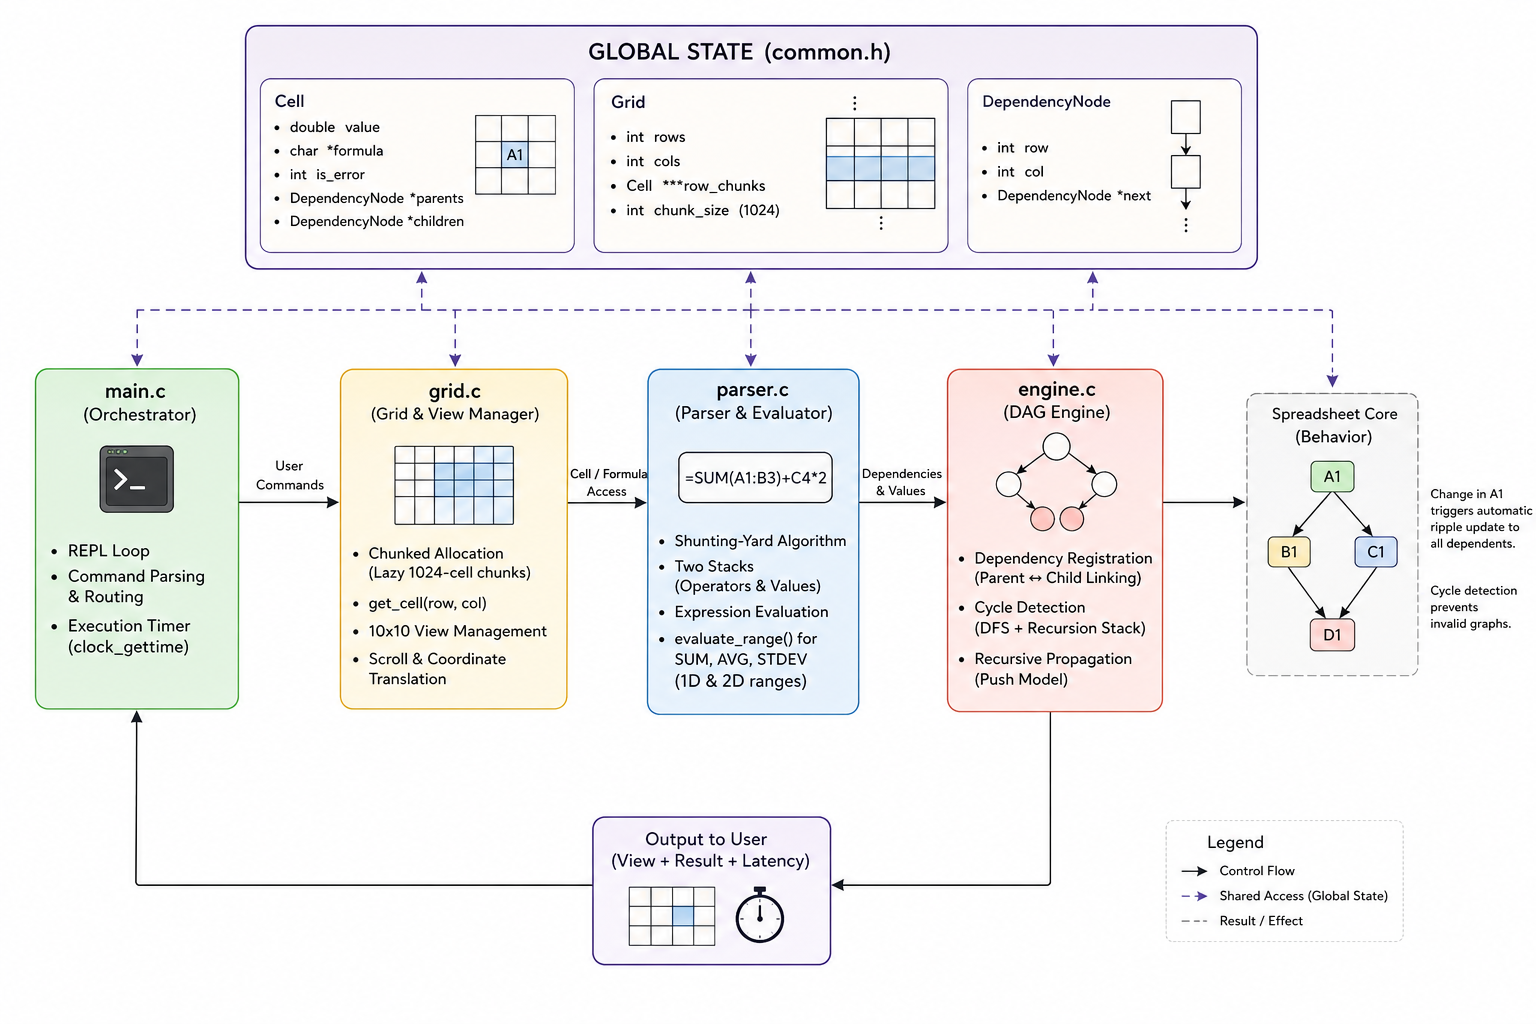
\includegraphics[width=\textwidth]{arch.png} 
    \caption{Spreadsheet System Architecture and File Dependencies}
    \label{fig:system_architecture}
\end{figure}
\section{GitHub Links}

\textbf{GitHub Repository:} \href{https://github.com/AyachiMishra/Ayachi_Swara_C_Project}{Ayachi\_Swara\_C\_Project}

\textbf{Commit History:} \href{https://github.com/AyachiMishra/Ayachi_Swara_C_Project/commits/main/}{Project Commit History}

\end{document}